\section{Discussion of Results}
Seismic hazard in northern Iran is computed based on background seismicity and projected on a set of hazard maps. The results obtained are represented as maps for the spatial distribution of horizontal peak ground acceleration with 10\% and 2\% probability of exceedance in 50 years, which correspond to the return period of 475 and 2475 years. The areas of large probabilistic ground motions clearly coincide with zones with a large number of events of magnitude 3.0 and larger. In this study we used two models for seismic hazard calculation, including $M_w>5$ and $M_w>4.5$. $M_w$ is the minimum magnitude that can affect the engineering site. In the probabilistic seismic hazard analysis increasing minimum magnitude will decrease the mean rate of earthquake occurrence ($\nu=exp(\alpha - \beta M_0)$), and also increase the value for the probability density function in the initial magnitudes. In a simple source the difference between different models specially in higher pga levels is negligible. However, in this study where we consider each event as a seismic source with different $\alpha$ and $\beta$ value, the results are considerably different. According to our results the reduction of the mean rate of earthquake occurrence has considerable effect on the results. 

\noindent
Results are presented for different models. In general in the models based on combination of five tectonic seismic regions there are five regions with high pga values. These regions are including: 40 km East of Gorgan (54.9,36.8), 50 km NW of Semnan(53.1,36), 110 km SW of Qazvin(48.9,35.8), 70 km SE of Ardabil(48.7,37.7), and 105 km North of Urmia(45.1,38.5). The pga values for each model at the mentioned places is presented in Table ~\ref{tab:pga_values_models}


\begin{table*}[!ht]
\centering
\caption{ Regions with higher Pga values (in g) for 5-regions model. }
\begin{tabular}{ cccccccccccccc}


	
	& & \multicolumn{6}{c}{10\% probability of exceedance in 50 years} & \multicolumn{6}{c}{2\% probability of exceedance in 50 years}    \\ 
	\cline{3-14}   & & \multicolumn{3}{c}{ $M_w > 5$ } & \multicolumn{3}{c}{ $M_w > 4.5$} & \multicolumn{3}{c}{ $M_w > 5$ } & \multicolumn{3}{c}{ $M_w > 4.5$ } \\ 
	\cline{3-14}    Lon & Lat & $-\sigma $ & $Mean$ & $+\sigma$ & $-\sigma $& $Mean$ &$+\sigma$& $-\sigma $ & $Mean$ & $+\sigma$& $-\sigma $ & $Mean$ & $+\sigma$ \\ \hline
	54.9	&	36.8	&	0.10	&	0.18	&	0.32	&	0.27	&	0.50	&	0.92	&	0.16	&	0.29	&	0.54	&	0.39	&	0.73	&	1.37 \\ \hline
	53.1	&	36.0 	&	0.09	&	0.16	&	0.28	&	0.26	&	0.47	&	0.85	&	0.14	&	0.27	&	0.51	&	0.38	&	0.71	&	1.31 \\ \hline
	48.9	&	35.8	&	0.09	&	0.16	&	0.28	&	0.24	&	0.44	&	0.79	&	0.15	&	0.28	&	0.52	&	0.37	&	0.68	&	1.24 \\ \hline
	48.7	&	37.7	&	0.07	&	0.14	&	0.26	&	0.23	&	0.42	&	0.76	&	0.14	&	0.25	&	0.46	&	0.36	&	0.66	&	1.20 \\ \hline
	45.1	&	38.5	&	0.06	&	0.11	&	0.20	&	0.20	&	0.38	&	0.72	&	0.11	&	0.20	&	0.38	&	0.34	&	0.61	&	1.08 \\ \hline
	 
\end{tabular}
\label{tab:pga_values_models}
\end{table*}








\noindent
Using different approaches, probabilistic seismic hazard analyses have been conducted for the northern Iran.
\citet{Tavakoli1999}, based on probabilisitic seismic computation using the historical and instrumental earthquake data, geology, tectonics, fault activity and seismic source model in Iran, prepared a new seismic hazard map of Iran. They divided Iran into 20 seismic tectonic regions and used seismic data up to 1997. They used \citet{Kijko1992} method  to determine the seismicity parameters.
The results were displayed for the return period of 75 and 475 years. They predicted the maximum mean acceleration, near north Tabriz fault zone, North Tehran fault zone, and Dasht-e-Bayaz fault zone, to be around 0.45g for return period of 475 years. The smallest value of 0.35g for 475 years is predicted in a narrow band trending NW-SE and extending from Urmia to Isfahan.  

\noindent
Using logic tree approach,\citet{Ghodrati2003} predicted the peak ground acceleration for Tehran for 475 years of return period. They used historical and instrumental data inside a circle of 200 km around the Tehran and converted them into $M_s$ magnitude scale. They used maximum likelihood method to get the seismicity parameters. Their results represented the peak ground acceleration for 10\% probability of exceedance in 50 years to be in range of $0.27g - 0.46g$.

\noindent
\citet{Ghodrati2008} studied seismic hazard and seismic zoning of Gilan province based on probabilistic approach. They used 3 attenuation relationship and 2 seismicity parameters through logic three approach. They presented the map of the maximum probable acceleration over bedrock for 475 and 2475 year return periods. The pga in the interested area, ranges from 0.1g to 0.3g and 0.2g to 0.45g for 475 and 2475 year return periods, respectively. 

\noindent
\citet{Vafaie2011} compiled a seismic catalog from 8th century A.D to 2006 for considering the near field effect earthquake PGA in Tabriz city in north-west of Iran. They used two attenuation relationships. They predicted the PGA for 475 and 2475 years of return period to be in range of 0.2 - 0.65 g and 0.3 - 0.9 g, respectively.  
\noindent
Using linear source model,\citet{Rahgozar2012} conducted a probabilistic assessment of PGA and uniform hazard spectra for Bojnurd city, the Capital of North Khorasan Province, Iran. They found the seismicity parameters of historical and instrumental data through \citet{Kijko2000} approach. They predicted the peak ground acceleration for three different attenuation relationships through implementing in the SEISRISK III software \citep{Bender1982}, and combine the results through logic tree approach. 
The results indicate that the PGA for 475 and 2475 years of return period will be in range of 0.15-0.22 g and 0.28-0.49 g, respectively.

\noindent
Using  EZ-FRISK computer program and considering $M_{min} = 4$ as a minimum magnitude that can affect the engineering site, \citet{Abdi2013} evaluated a probabilistic seismic hazard analysis for Tehran and surrounding areas in order to quantify the dominant events that have the most contribution on ground motion exceedance from different hazard level. They predicted the PGA for Tehran and Karaj city to be in range of 0.27 - 0.3 g for return period of 475 years. 

\noindent
\citet{Abdollahzadeh2014a} carried out a probabilistic seismic hazard assessment for part of Northern Iran. They used the logic tree approach to capture the epistemic uncertainty of seismic hazard assessment in delineation of seismic sources and selection of attenuation relationship. They used three attenuation relationships and 2 seismic source models. They collected the earthquake catalog from various references and reported the pga for 475 and 2475 years of return period for northern cities.   

\noindent
\citet{Golara2014} conducted a probabilistic seismic hazard analysis of interconnected infrastructure of Iranian high pressure gas supply system. He used line and area source model in order to estimate the Iranian  high-pressure gas supply system's ability to withstand a sudden large ground movements caused by potential earthquakes and related phenomenon that might be expected. he used simplified tectonic map after \citet{Alavi1991}. He used four attenuation relationships and presented the results for 2475 years of return period. 

\noindent
\citet{Boostan2015} developed new model for probabilistic seismic hazard assessment based on fuzzy sets theory for Tehran, Iran. The results is about 0.42-0.48 g for 475 years. 

Table ~\ref{tab:pga_values} presents the PGA value for some of the major cities in northern Iran from different studies. This study values are results of 5-region model with $M_w > 4.5 $.



\begin{table*}[!ht]
\centering
\caption{Comparison of PGA, from different studies for selected cities in Northern Iran. This study values are results of 5-regions model with "$M_w > 4.5$" (V2011:  \citet{Vafaie2011}), G2008: \citet{Ghodrati2008}, B2015: \citet{Boostan2015},  G2003:  \citet{Ghodrati2003},  Az2014: \citet{Abdollahzadeh2014a} , Ra2012: \citet{Rahgozar2012} , Ab2013: \citet{Abdi2013} ) }
\begin{tabular}{ | c | c | c | c | c | c | c | c | c | c | c |}


\hline

	
	\multirow{2}{*}{Cities} & \multirow{2}{*}{Lon} & \multirow{2}{*}{Lat} & \multicolumn{2}{|c|}{This study} & \multirow{2}{*}{2800} & Zare & Golara &\multicolumn{3}{|c|}{Other Refrences}    \\ 
	\cline{4-5}  \cline{9-11}  &  &  & 10\% & 2\% &  &  2012 & 2014 & 10\% & 2\% & ref \\ \hline
	 Urumieh   & 45.1   & 37.6    & 0.25 & 0.41   & 0.3 & 0.35-0.5 & 0.3-0.5 &  &  &  \\ \hline
	 Tabriz       & 46.3    & 38.1   & 0.23 & 0.39   & 0.35 & 0.35-0.5 & 0.9-1.2& 0.2- 0.65 & 0.3 to 0.9 & V2011 \\ \hline
	 Ardabil      & 48.3   & 38.3   & 0.30 & 0.51    & 0.3 & 0.35-0.5 &0.5-0.7  &&  &  \\ \hline
	 Zanjan      & 48.5   & 36.7   & 0.19 & 0.32    & 0.3 & 0.35-0.5 &0.5-0.7  &&  &  \\ \hline
	 Manjil       & 49.4   & 36.7    & 0.33 & 0.53   & 0.35 & 0.65 $<$ &0.5-0.7& 0.25 & 0.4 & G2008 \\ \hline
	  \multirow{2}{*}{Rasht}  & \multirow{2}{*}{49.6} & \multirow{2}{*}{37.3} & \multirow{2}{*}{0.3} & \multirow{2}{*}{0.5} & \multirow{2}{*}{0.3} & \multirow{2}{*}{0.5-0.65} & \multirow{2}{*}{0.5-0.7} & 0.1 &  0.2 &  G2008 \\ 
	  \cline{9-11}	             &  &  &  &  &  &  & & 0.25-0.3 & 0.55-0.6 & Az2013\\ \hline
	 Qazvin     & 50.0   & 36.3    & 0.22 & 0.37   & 0.35 & 0.35-0.5 &0.5-0.7& 0.31 & 0.42 &  \\ \hline
	 Karaj        & 51.0   & 35.8    & 0.20 & 0.36   & 0.35 & 0.35-0.5 &0.7-0.9& 0.31 & 0.42 & Ab2013 \\ \hline
	 \multirow{3}{*}{Tehran}  & \multirow{3}{*}{51.4} & \multirow{3}{*}{35.7} & \multirow{3}{*}{0.27} & \multirow{3}{*}{0.45} & \multirow{3}{*}{0.35} & \multirow{3}{*}{0.35-0.5} & \multirow{3}{*}{0.7-0.9} & 0.37-0.42 &  &  G2003 \\ 
	 \cline{9-11}	             &  &  &  &  &  &  & & 0.27-0.3  &  & Ab2013\\ 
	 \cline{9-11}	             &  &  &  &  &  &  & & 0.42-0.48 &  & B2015\\ \hline
	 Sari          & 53.0   & 36.3   & 0.39   & 0.62  & 0.3 & 0.35-0.5 &0.5-0.7& 0.3 - 0.35 &  0.65 - 0.7 & Az2014\\ \hline
	 Semnan   & 53.4   & 35.6   & 0.36   & 0.55  & 0.3 & 0.35-0.5 &0.3-0.5&  & & \\ \hline
	 Gorgan    & 54.4   & 36.8    & 0.45  & 0.69  & 0.3 & 0.35-0.5 &0.5-0.7& 0.3 - 0.35 &  0.65 -0.7 & Az2014\\ \hline
	 Bojnurd   & 57.3    & 37.5    & 0.43  & 0.67  & 0.3 & 0.35-0.5 &0.7-0.9&0.16-0.2  & 0.32-0.45  & Ra2012  \\ \hline
	 Mashhad & 59.6     & 36.3   & 0.21 & 0.37  & 0.3 & 0.35-0.5 &0.7-0.9  &  &&  \\ \hline
 
\end{tabular}
\label{tab:pga_values}
\end{table*}



\subsection{$\pm \sigma$ of attenuation relationship}
In this study we use one attenuation relationship (See the discussion in the attenuation relationship section). In order to consider the uncertainty of the ground motion equation we also present the $\pm$ standard deviation of each seismic hazard model. These figures give an idea about the range of probable peak ground acceleration for 10\% and 2\% probability of exceedance in 50 years. Fig.~\ref{fig:pga_10_minus_plus} and Fig.~\ref{fig:pga_2_minus_plus} show the results of plus and minus standard deviation of attenuation relationship, respectively. These figures show the variation of peak ground acceleration for each model. However, due to inability of the earth to carry more intense seismic waves, there is almost certainly some true physical upper bound on ground motion intensity \citep{Baker2008}


\begin{figure*} [!ht]
\centering
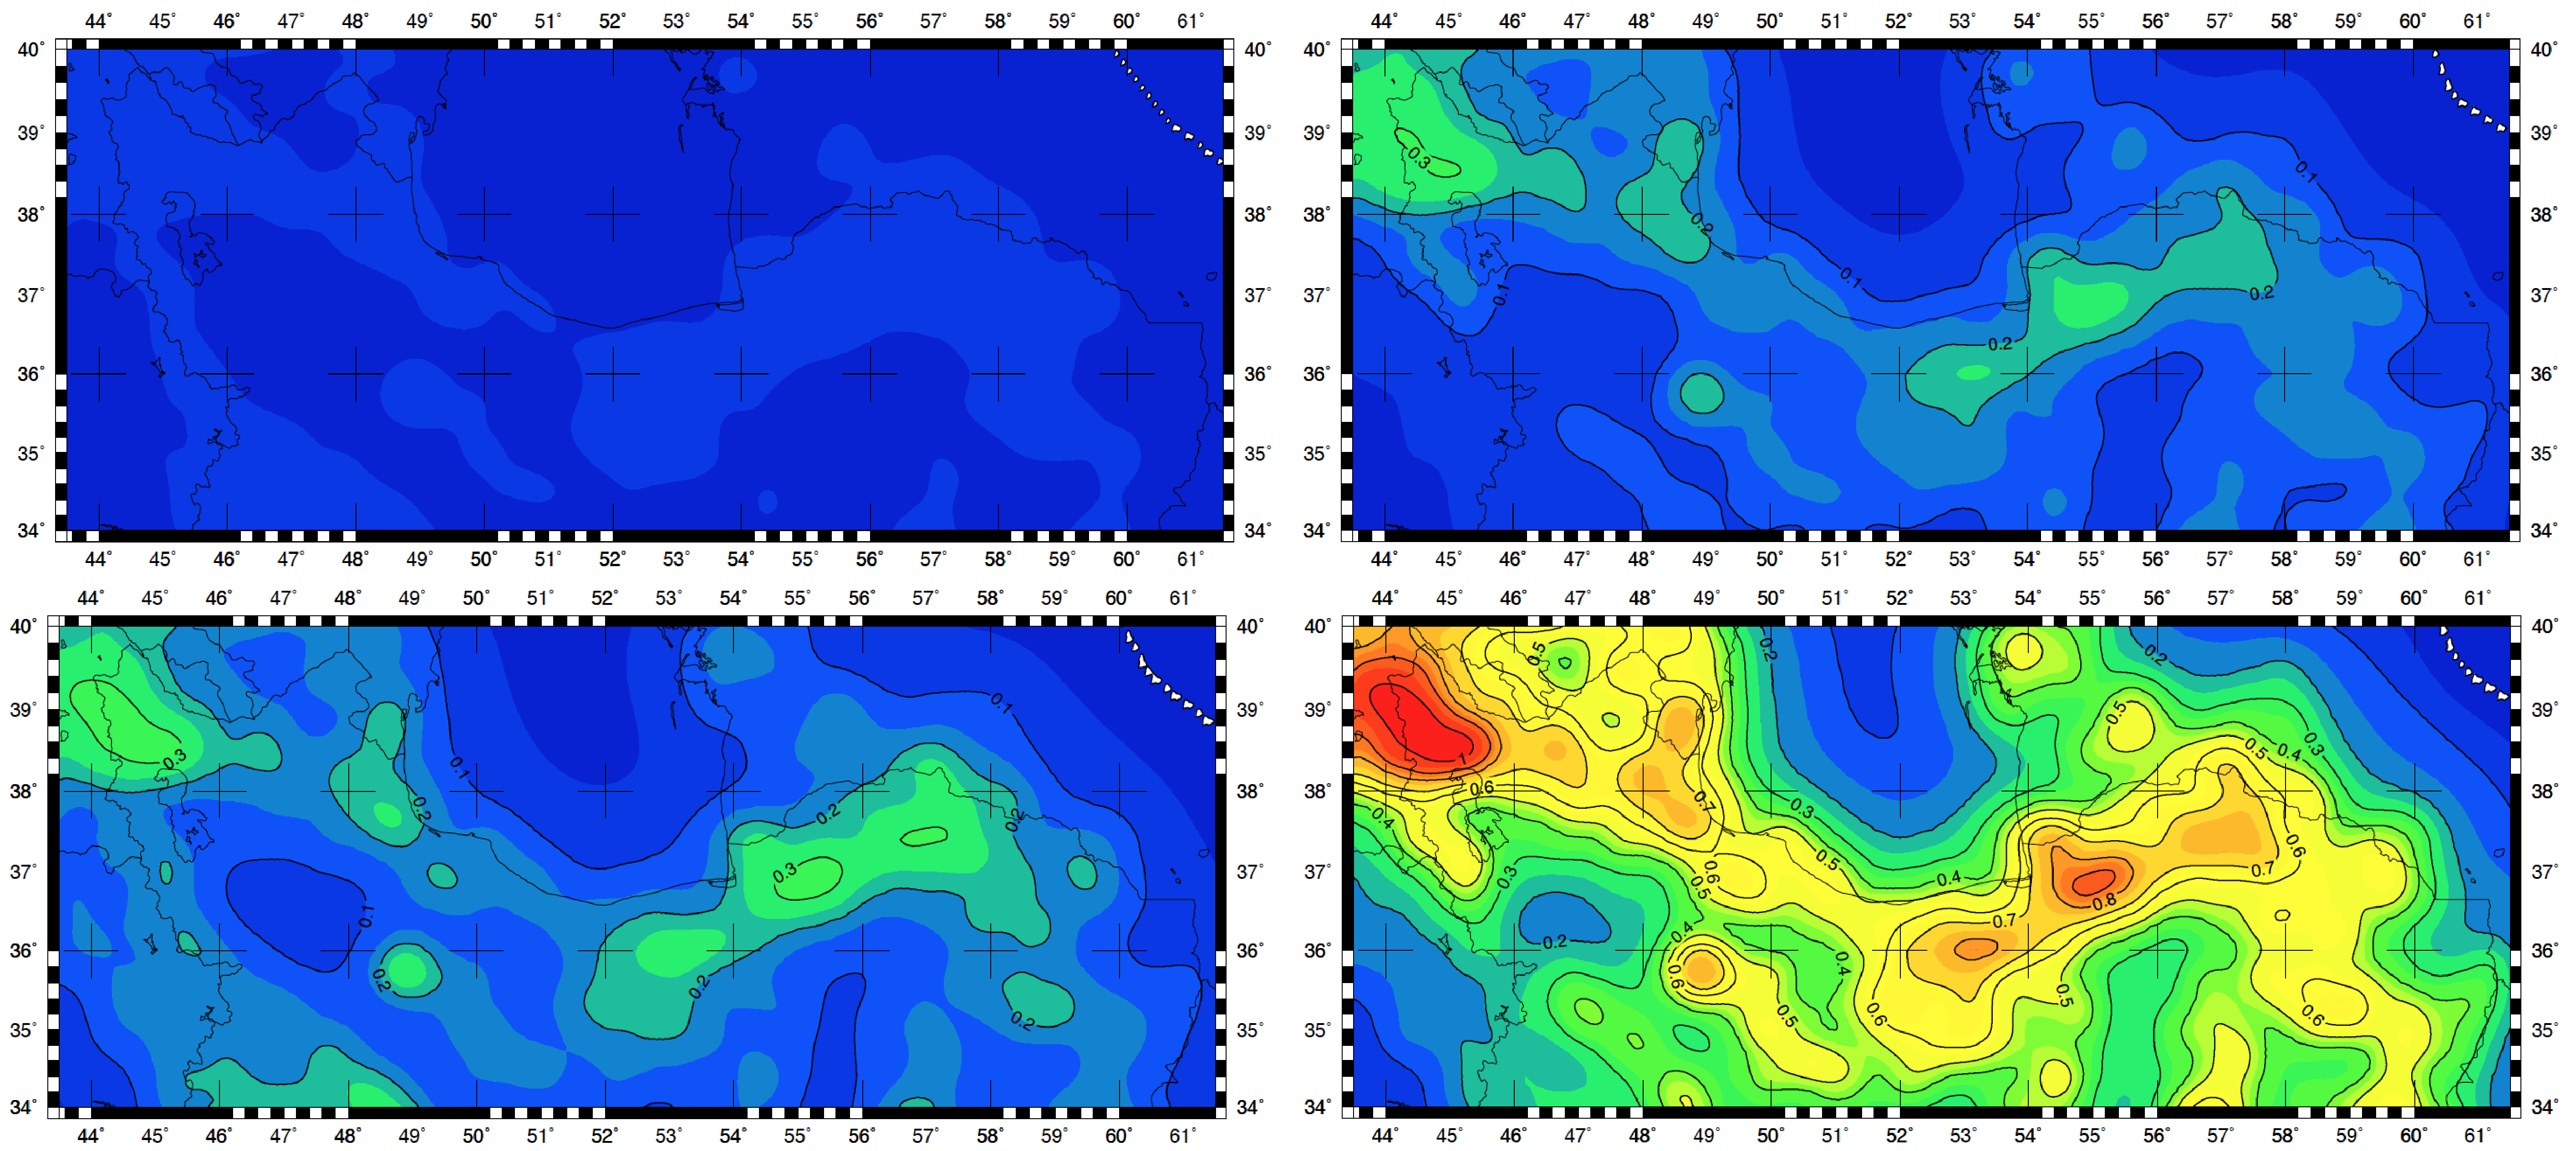
\includegraphics[scale=0.15]{figures/pdf/pga_10_minus_plus.pdf} 
\caption{$\pm$ standard deviation of peak ground acceleration for 10\% probability of exceedance in 50 years.}
\label{fig:pga_10_minus_plus}
\end{figure*}


\begin{figure*} [!ht]
\centering
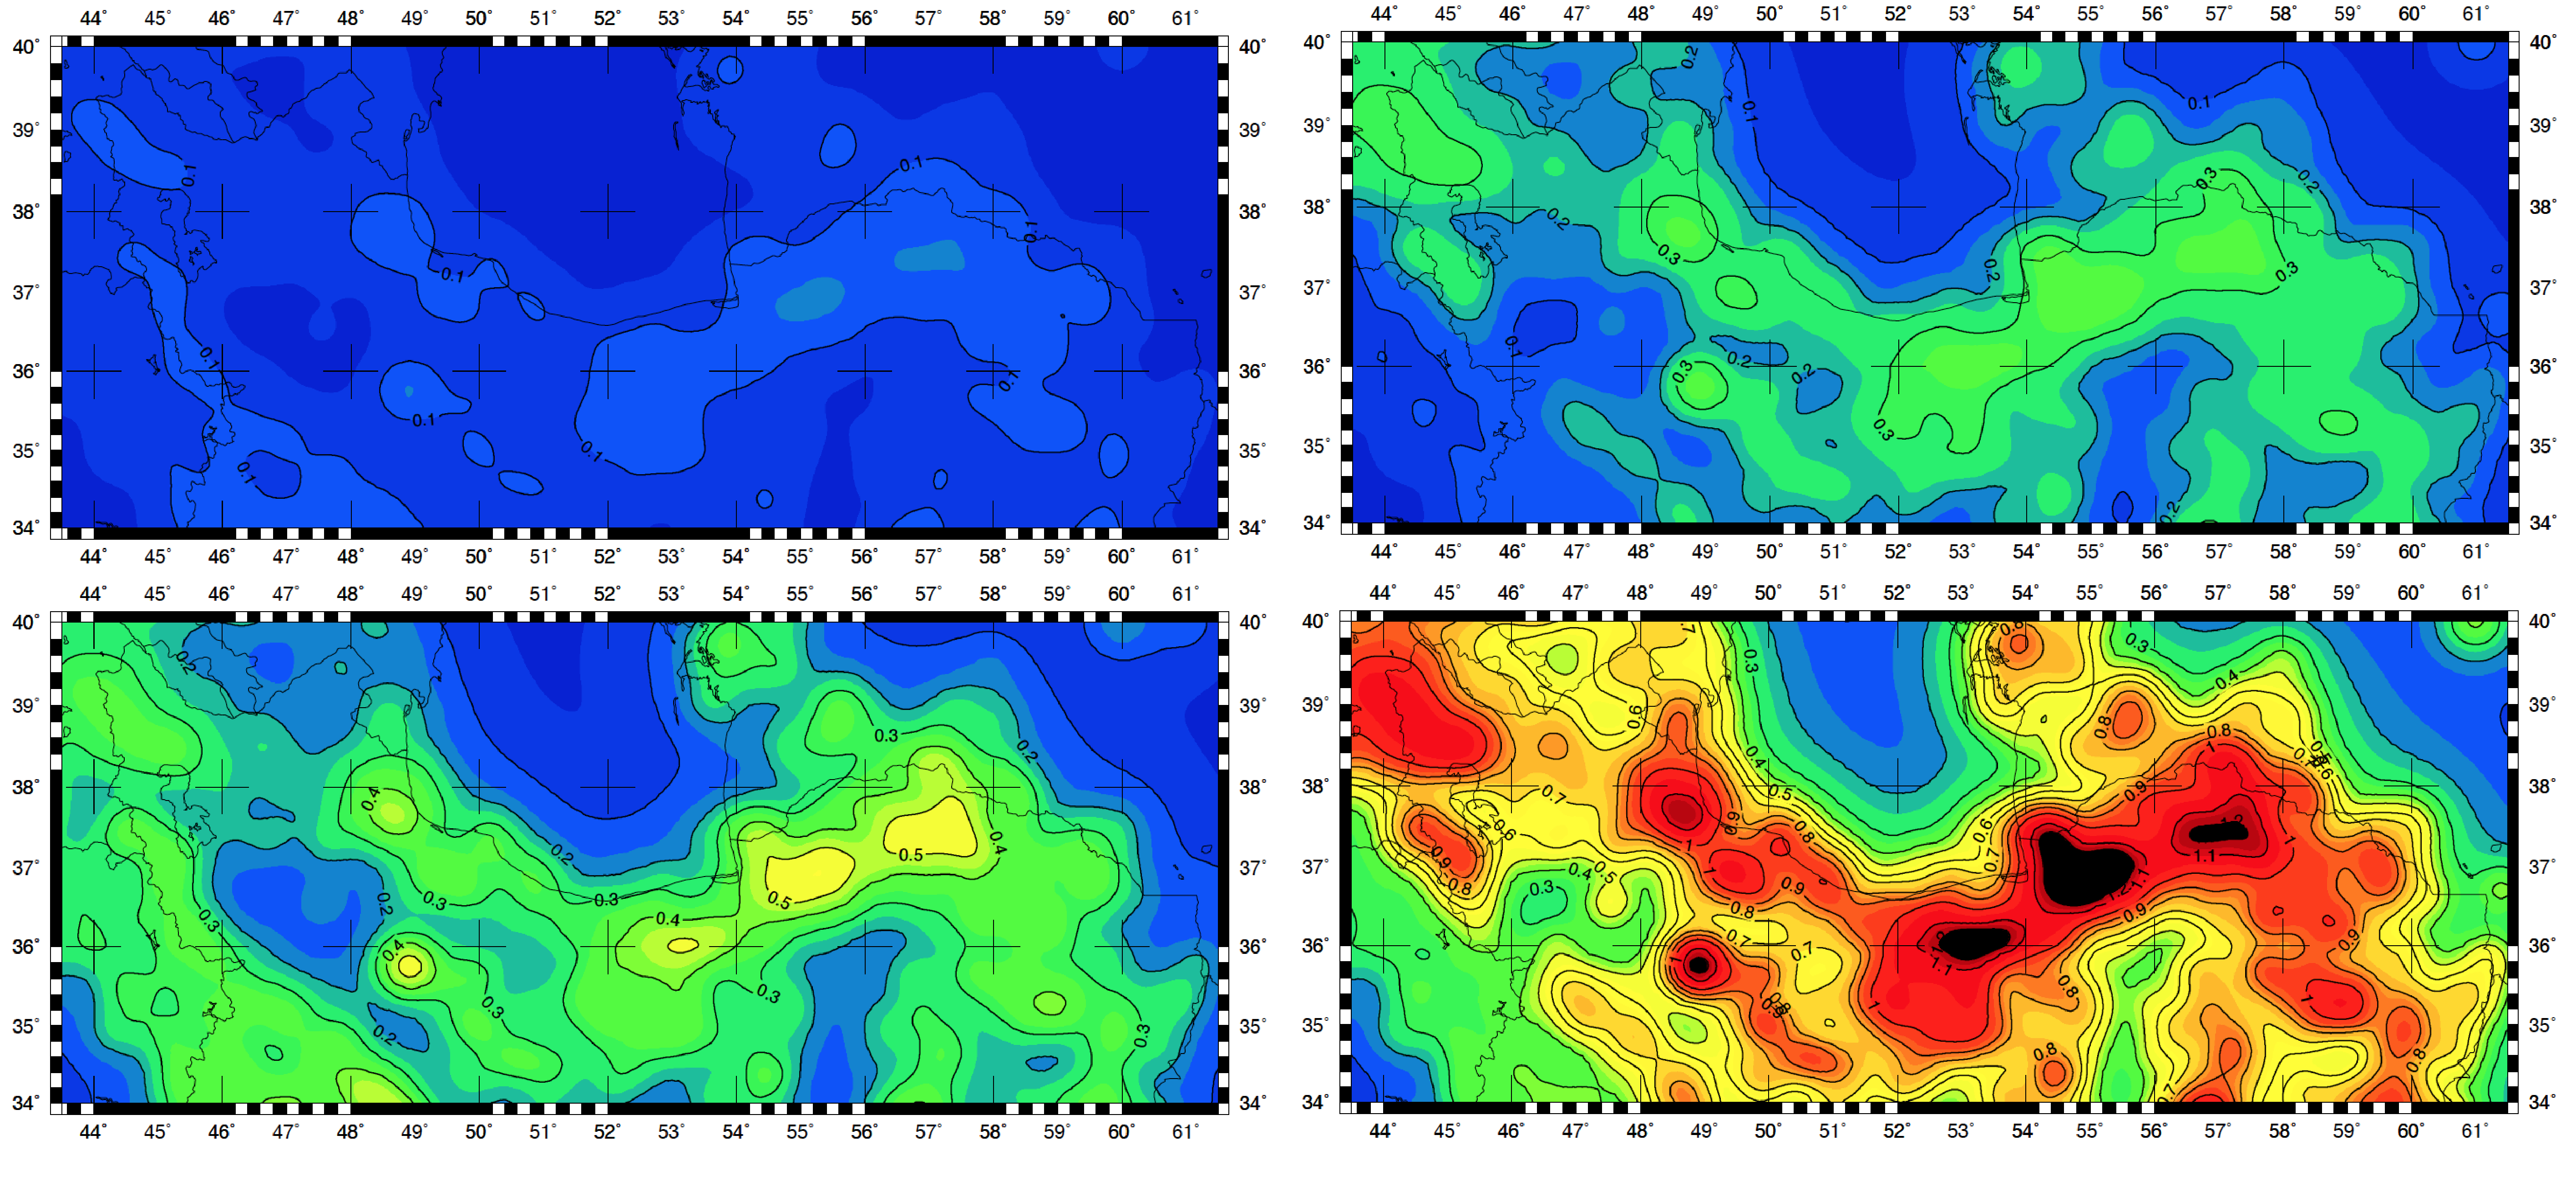
\includegraphics[scale=0.15]{figures/pdf/pga_2_minus_plus.pdf} 
\caption{$\pm$ standard deviation of peak ground acceleration for 2\% probability of exceedance in 50 years.}
\label{fig:pga_2_minus_plus}
\end{figure*}



%\subsection{30-70}
%\subsection{Hazard Curve}
